\documentclass[11pt]{beamer}

\usetheme{metropolis}

\usepackage{graphicx}
\usepackage{physics}
\usepackage{adjustbox}
\usepackage{caption}
\usepackage{chemformula}
\usepackage{quoting}
\usepackage[style=chem-angew,backend=bibtex]{biblatex}
\bibliography{references}
%
% Choose how your presentation looks.
%
% For more themes, color themes and font themes, see:
% http://deic.uab.es/~iblanes/beamer_gallery/index_by_theme.html
%
\mode<presentation>
{
  \usetheme{default}      % or try Darmstadt, Madrid, Warsaw, ...
  \usecolortheme{default} % or try albatross, beaver, crane, ...
  \usefonttheme{default}  % or try serif, structurebold, ...
  \setbeamertemplate{navigation symbols}{}
  \setbeamertemplate{caption}[numbered]
  \setbeamerfont{footnote}{size=\tiny}
} 

\usepackage[english]{babel}
\usepackage[utf8]{inputenc}
\graphicspath{{../lectureMW/image/}}

\AtBeginSection[]{
\begin{frame}{Outline}
  \tableofcontents[currentsection]
\end{frame}
}

\title{Chapter 7: Electromagnetic Radiation (Light Energy)}
\institute{Chemistry Department, Cypress College}
\date{November 10, 2022}

\begin{document}

\begin{frame}
  \titlepage
\end{frame}

\begin{frame}{Class Announcements}
  \textbf{Lecture}
  \begin{itemize}
  \item Review Chemical Equations and Limiting Reagent problems
  \item Work in groups and present the exam problems
    (If we finish, everyone receive 2 EC pt in lieu of HW presentations)
  \item Ch 7 - Electromagnetic Radiation
  \item Quiz and Homework assignment released Fri, Nov 4th at 3pm
  \end{itemize}
\end{frame}

\section{Light Energy}

\begin{frame}{Photosynthesis Harnesses Light}
  \centering
  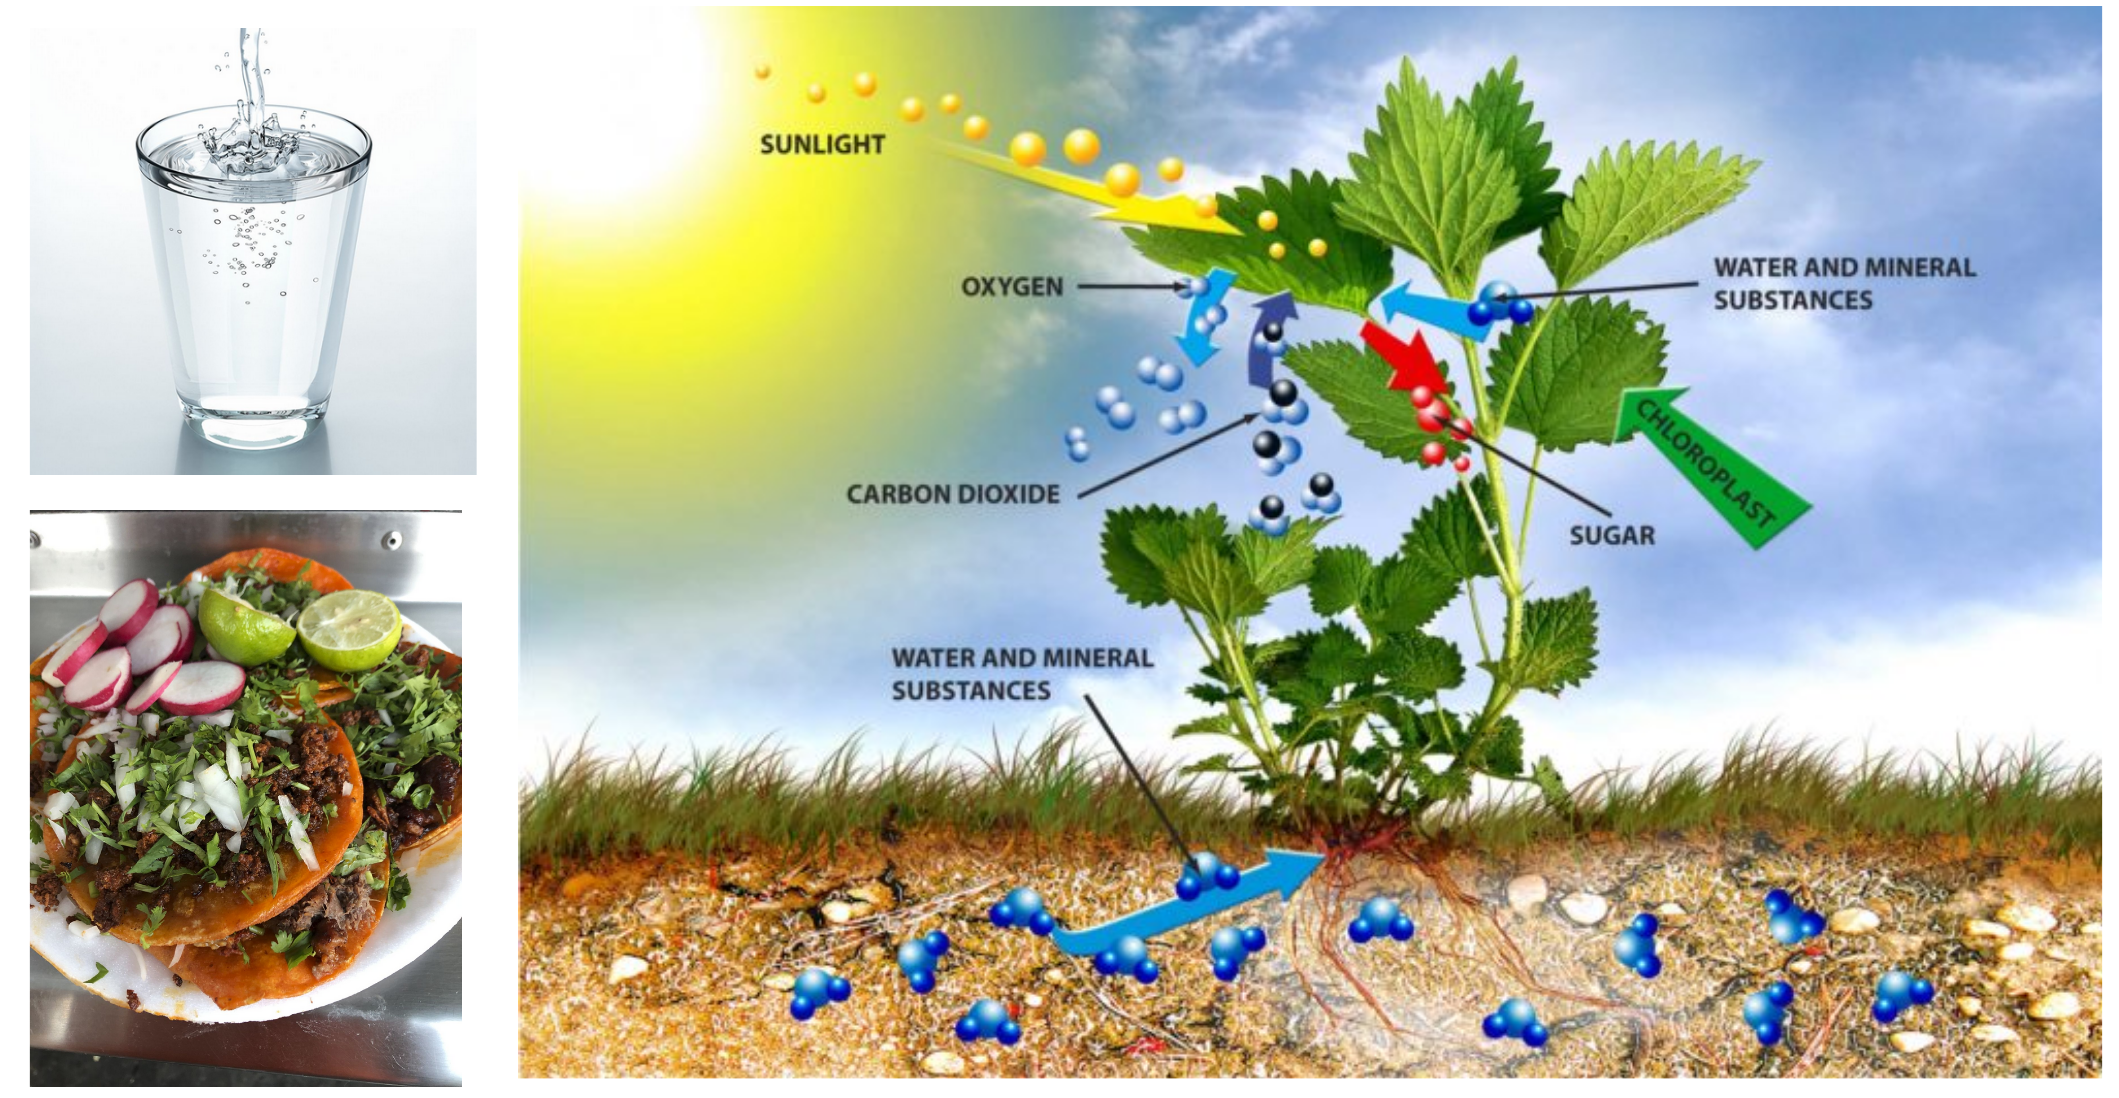
\includegraphics[trim={8in 0 0 0},clip,width=1\linewidth]{food_pic}
\end{frame}

\begin{frame}{Electromagnetic Radiation}
  \centering
  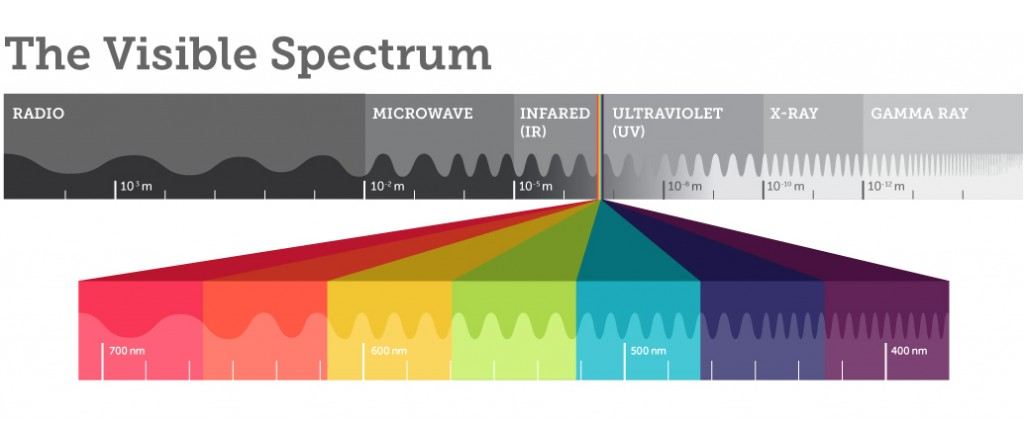
\includegraphics[width=0.85\linewidth]{visible_light}
  
  Visible light range from 700nm to 400nm;
  ROYGBV
  
  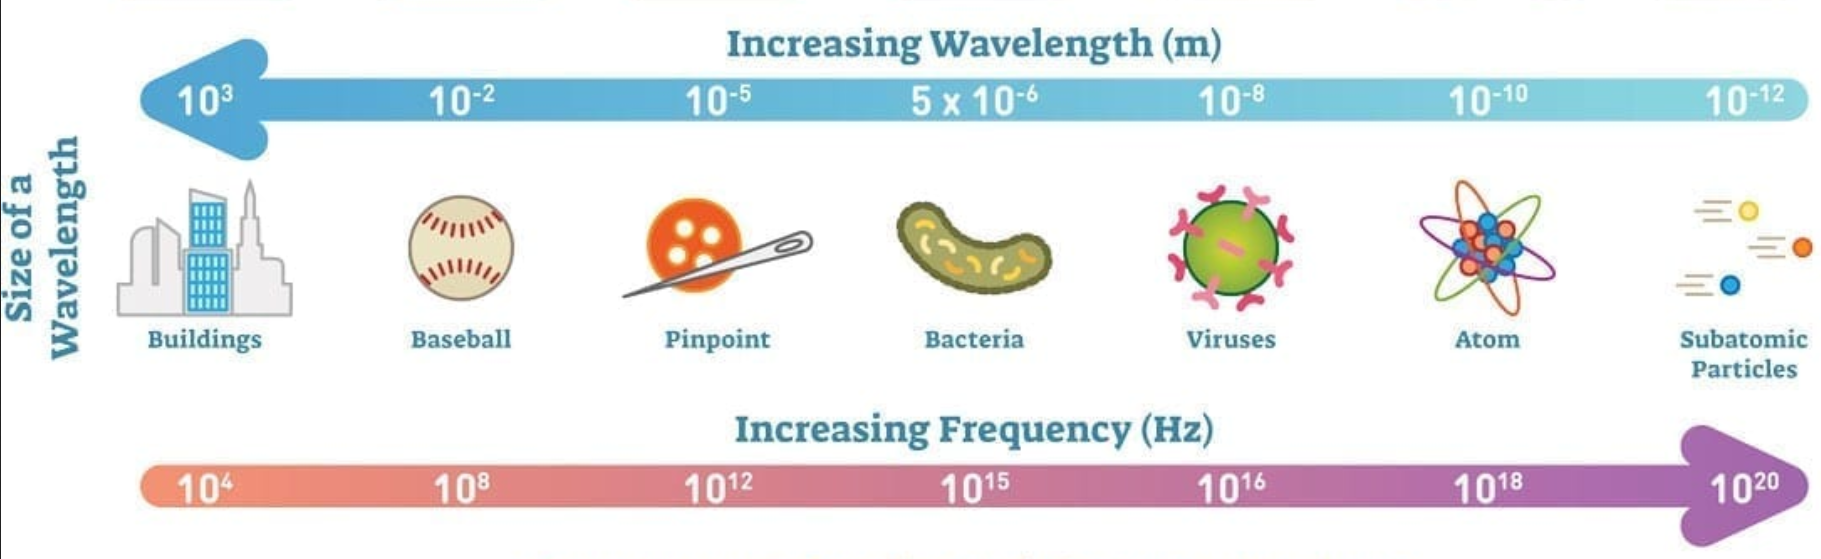
\includegraphics[width=0.85\linewidth]{wave_freq_size}
\end{frame}

\begin{frame}{Radiation Energy}
  \begin{center}
    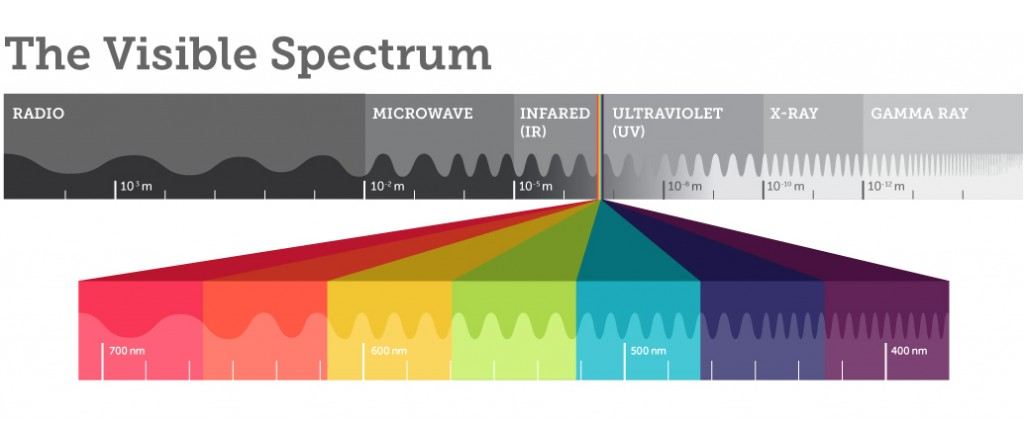
\includegraphics[width=0.85\linewidth]{visible_light}
  \end{center}
  \begin{equation}
    E = \frac{hc}{\lambda}
    \label{eqn:photon}
  \end{equation}
  where $\lambda$ is the wavelength (m), $c$ is the speed
  of light ($3.00 \times 10^8$ m/s), $h$ is the Planck constant
  ($6.626 \times 10^{-34}$ J s) and $E$ is energy (J)
\end{frame}

\begin{frame}{Practice: Photosynthesis}
  Chloroplast absorbs mostly violet (450 nm) and red (650 nm) light
  while reflecting green. What is the corresponding energies in J
  for these colors?
  \vspace{1.75in}
\end{frame}

\begin{frame}{Where light energy comes from?}
  \centering
  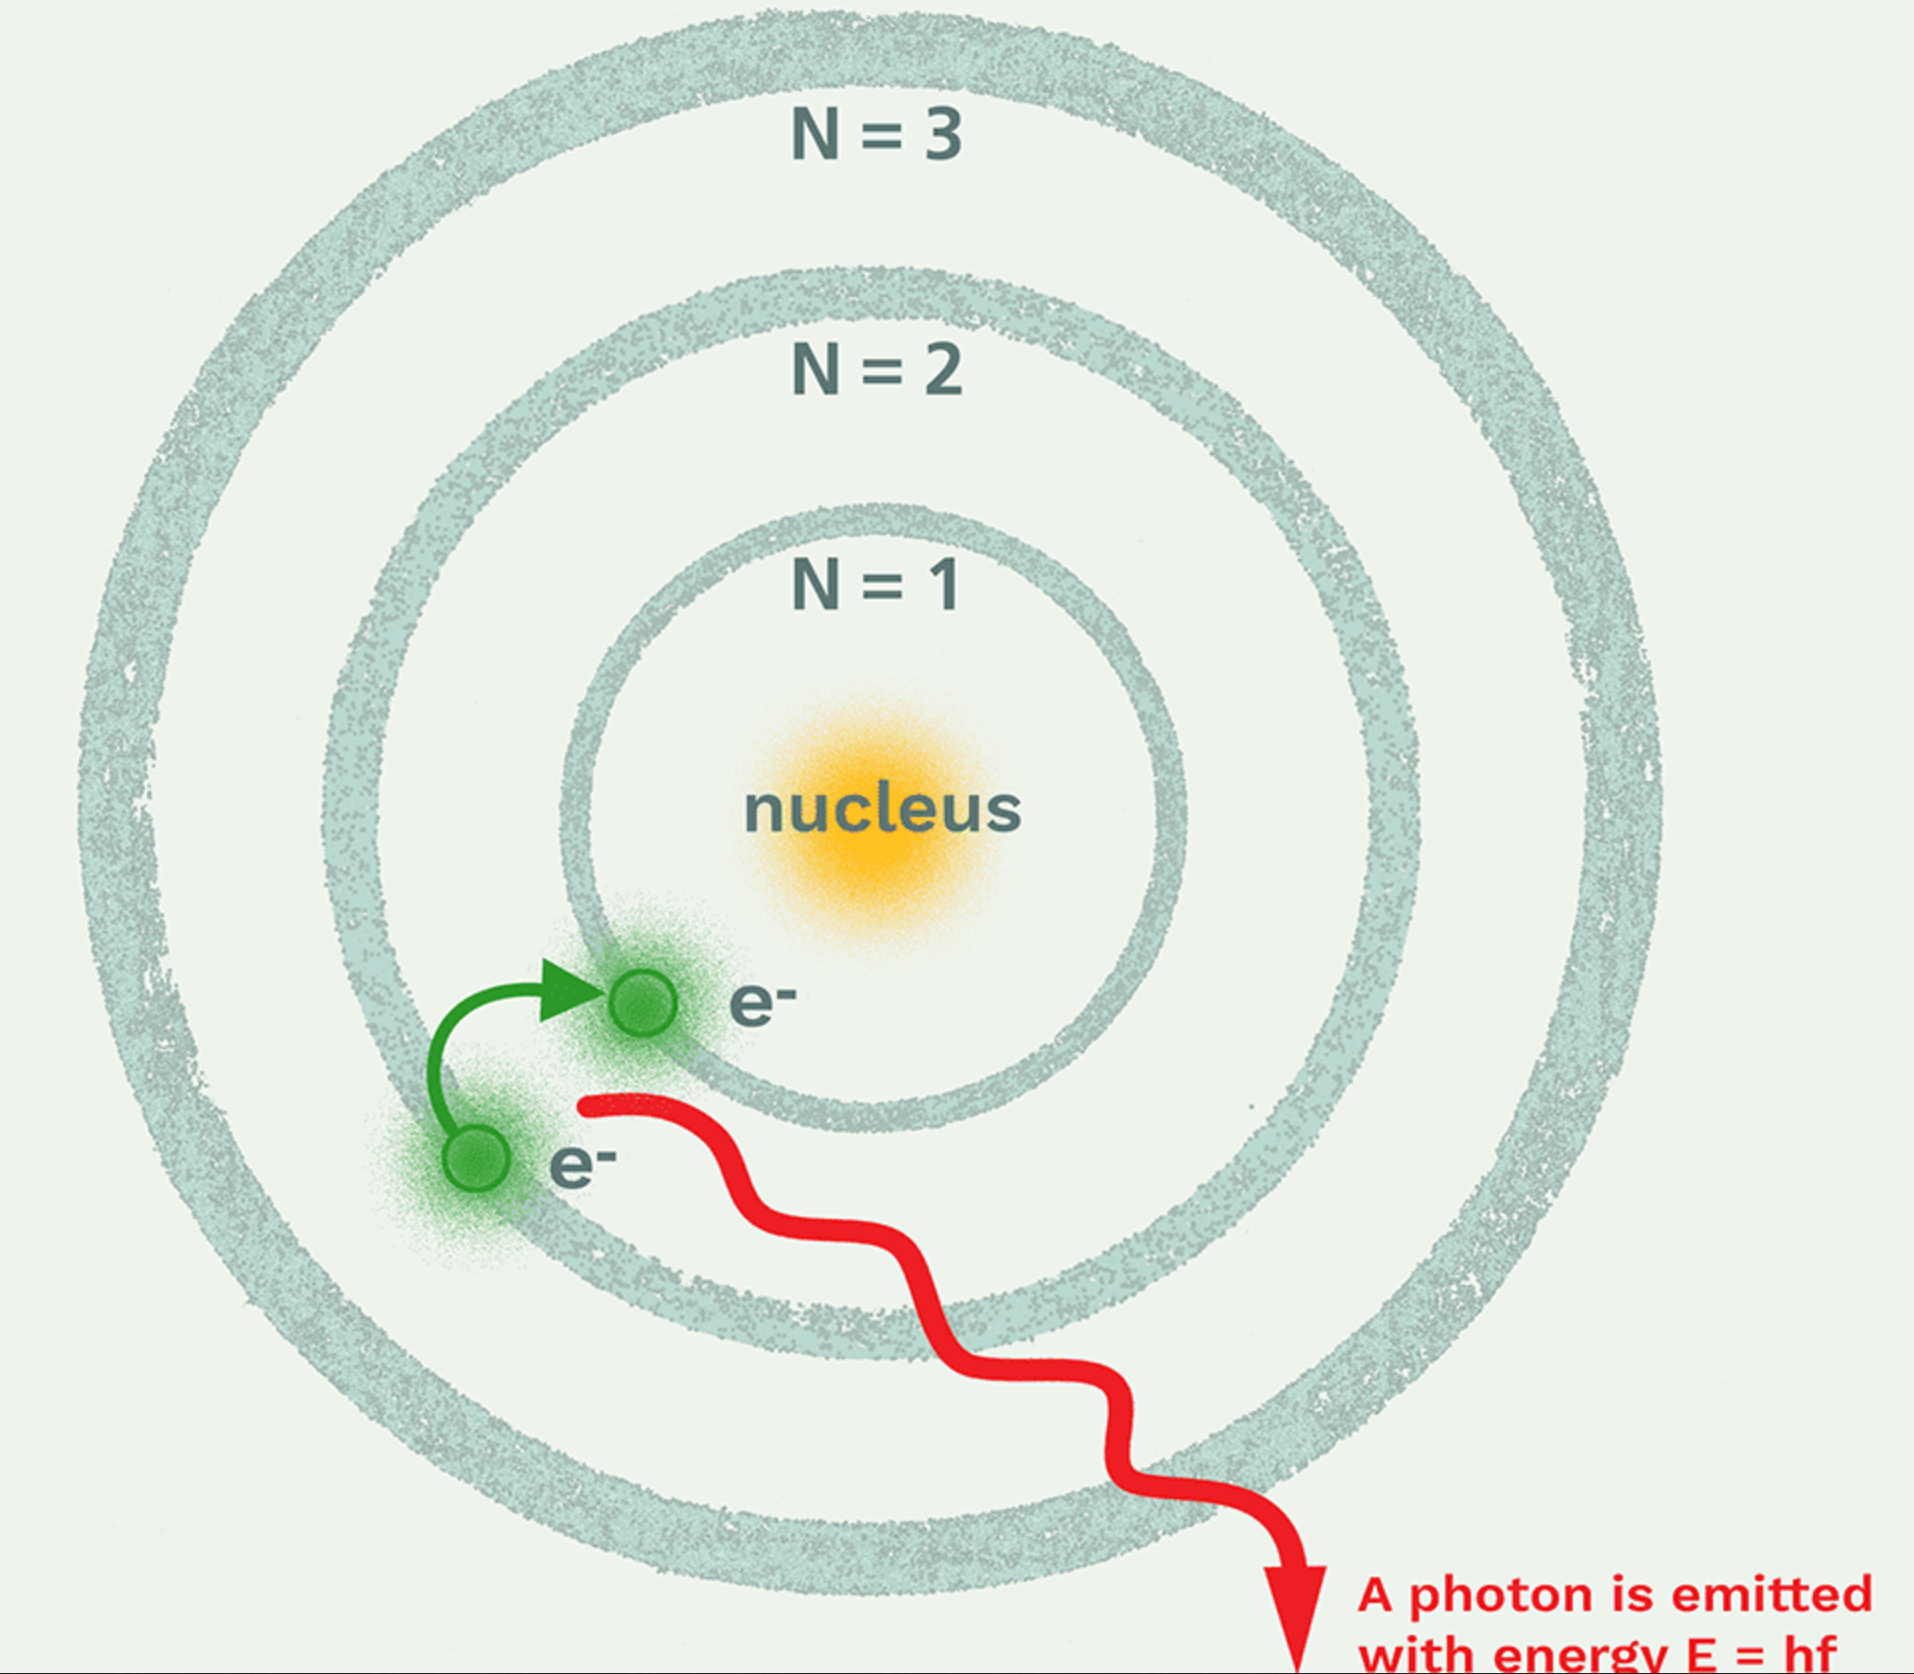
\includegraphics[width=0.55\linewidth]{bohr_model}
  
  \href{https://www.youtube.com/watch?v=IXxZRZxafEQ}{Youtube Link: What is Light?}
\end{frame}

\begin{frame}{Atomic Spectra}
  \centering
  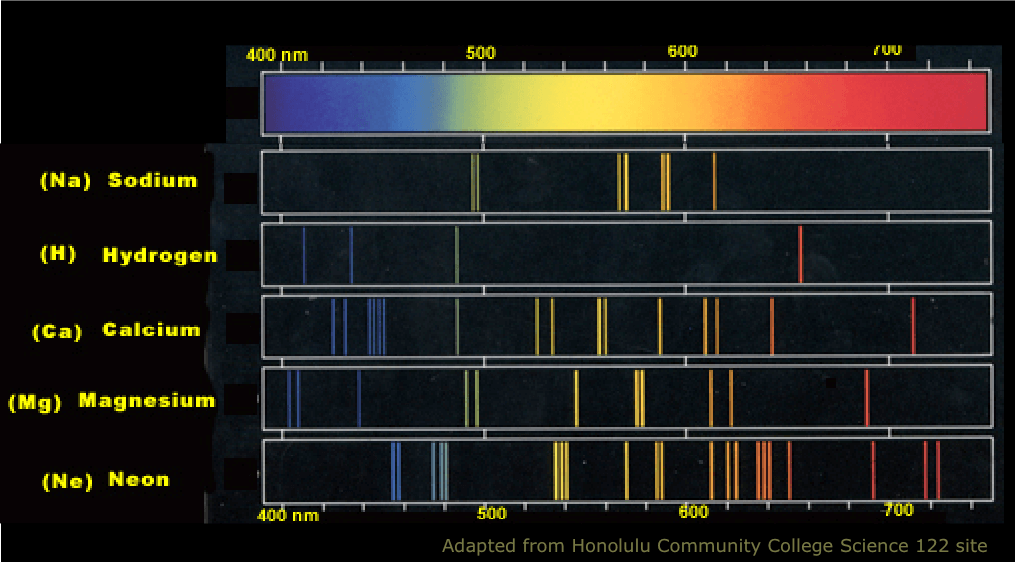
\includegraphics[width=0.85\linewidth]{cont_line}
  \begin{itemize}
  \item Continuous spectra is given at the top and
    discrete lines are emitted by atoms
  \item \textbf{Q:} Why are there discrete lines for
    the atomic spectra?
  \end{itemize}
\end{frame}

\section{Periodicity of Electron Configurations}

\begin{frame}{Describing the Atom: Bohr Model}
  \centering
  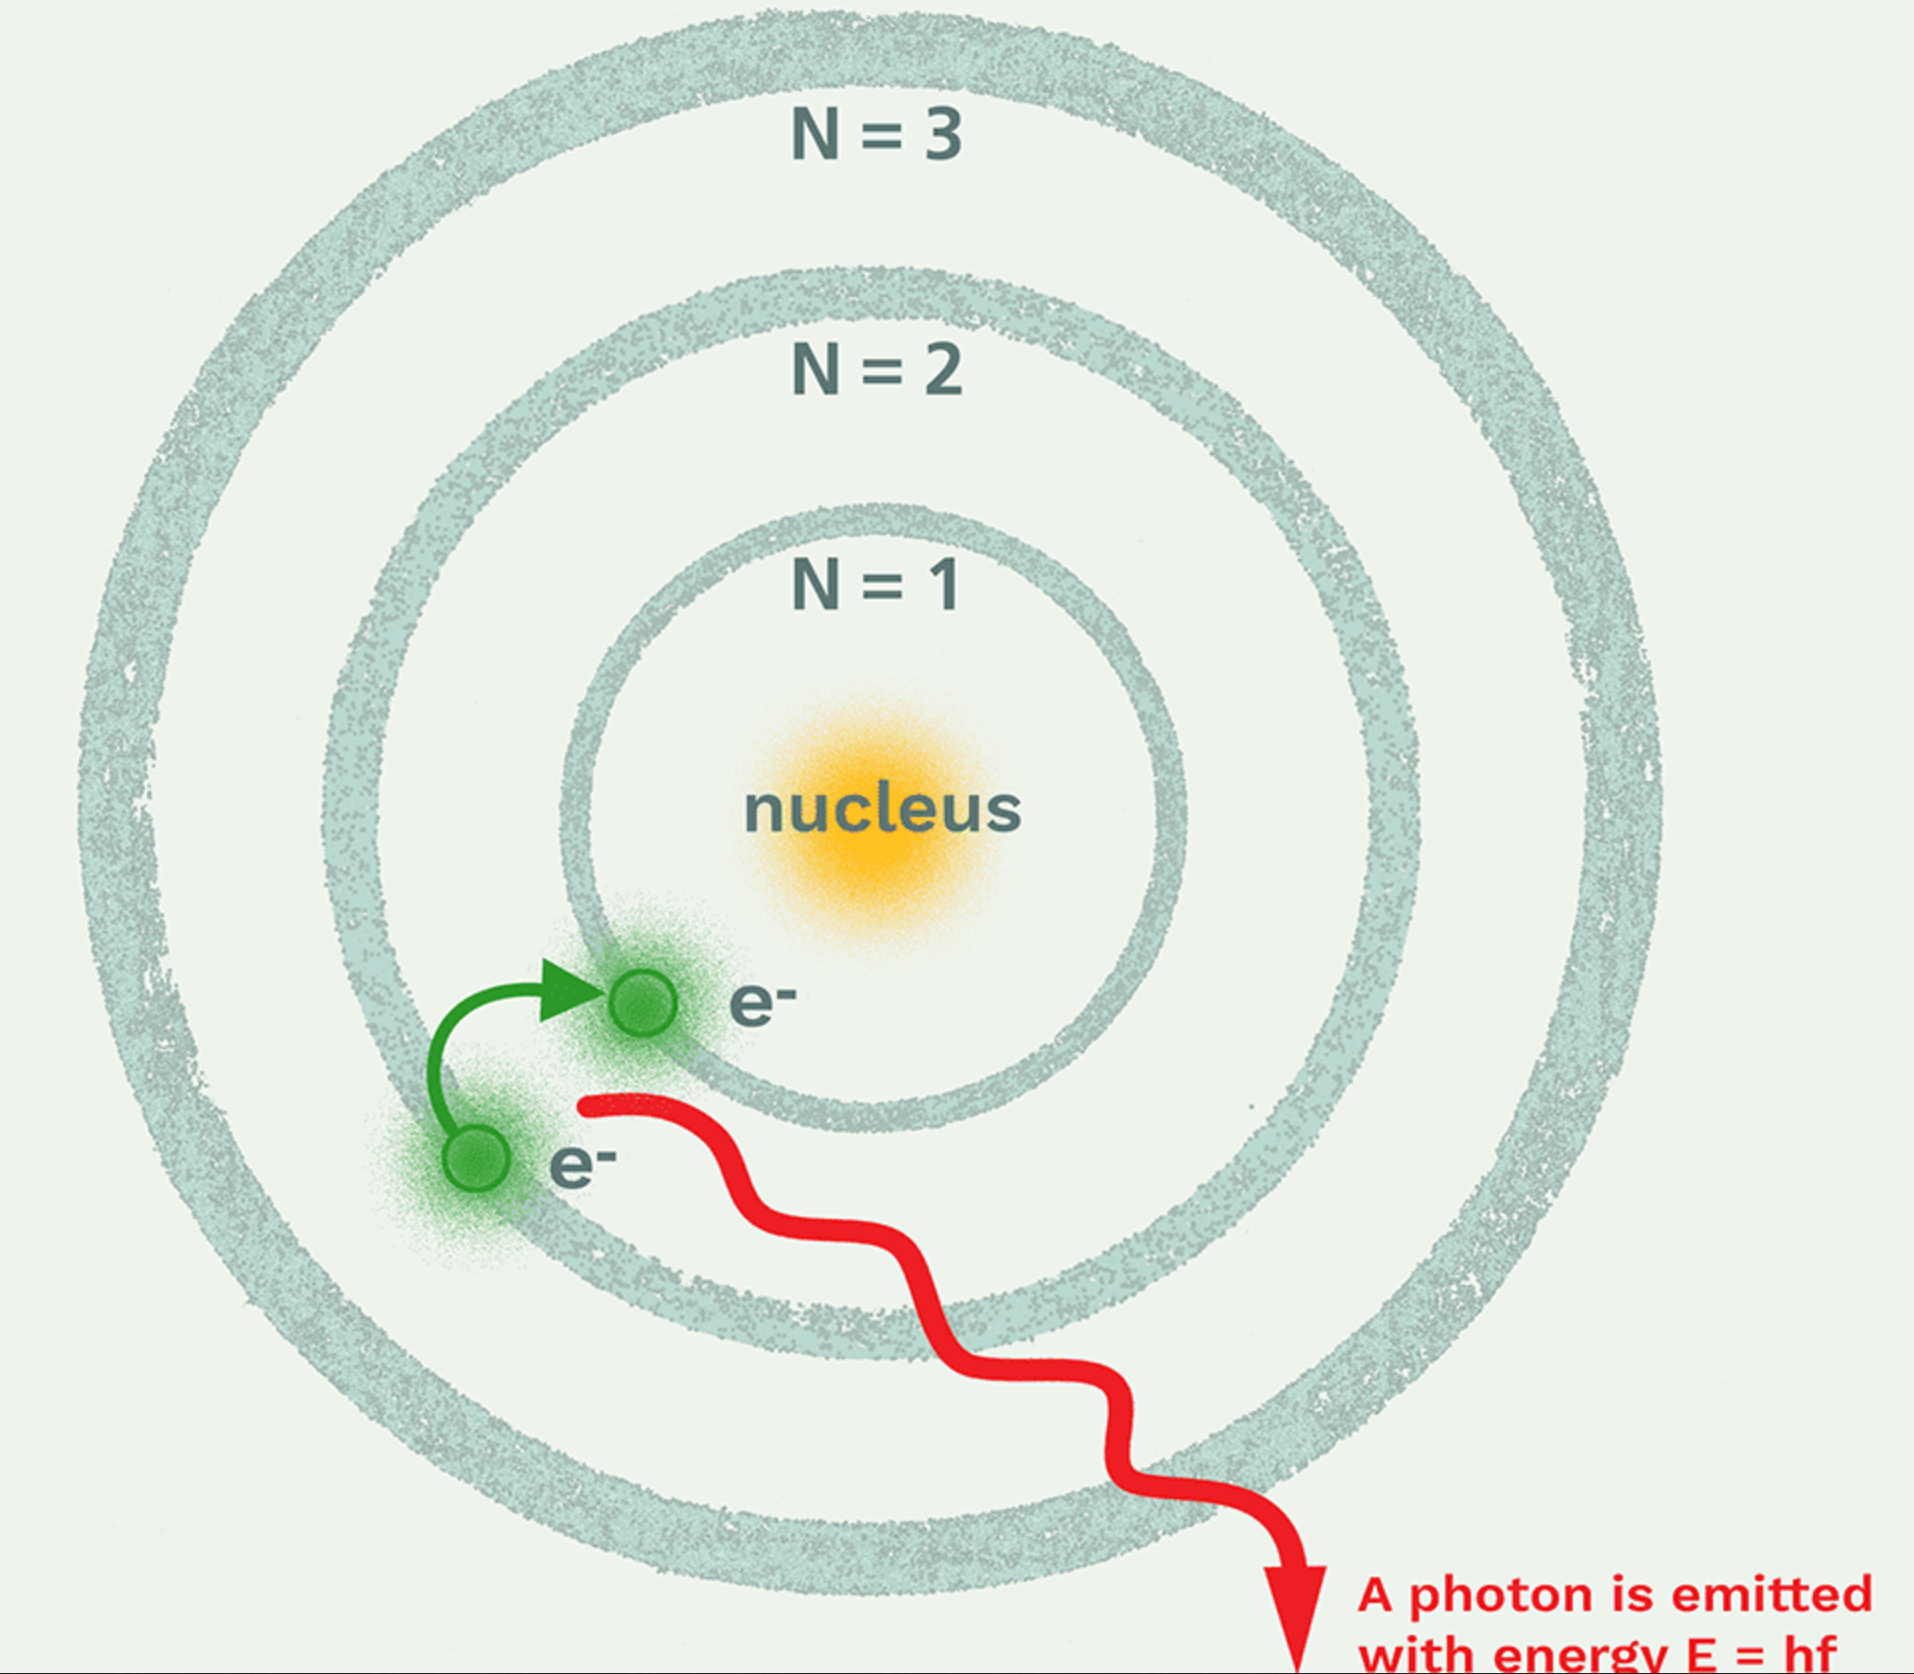
\includegraphics[width=0.55\linewidth]{bohr_model}
  \begin{itemize}
  \item Energy is quantized
  \item Electronic energy is proportional to the size of
    the orbit
  \end{itemize}
\end{frame}

\begin{frame}{Describing the Atom: Atomic Orbitals}
  \centering
  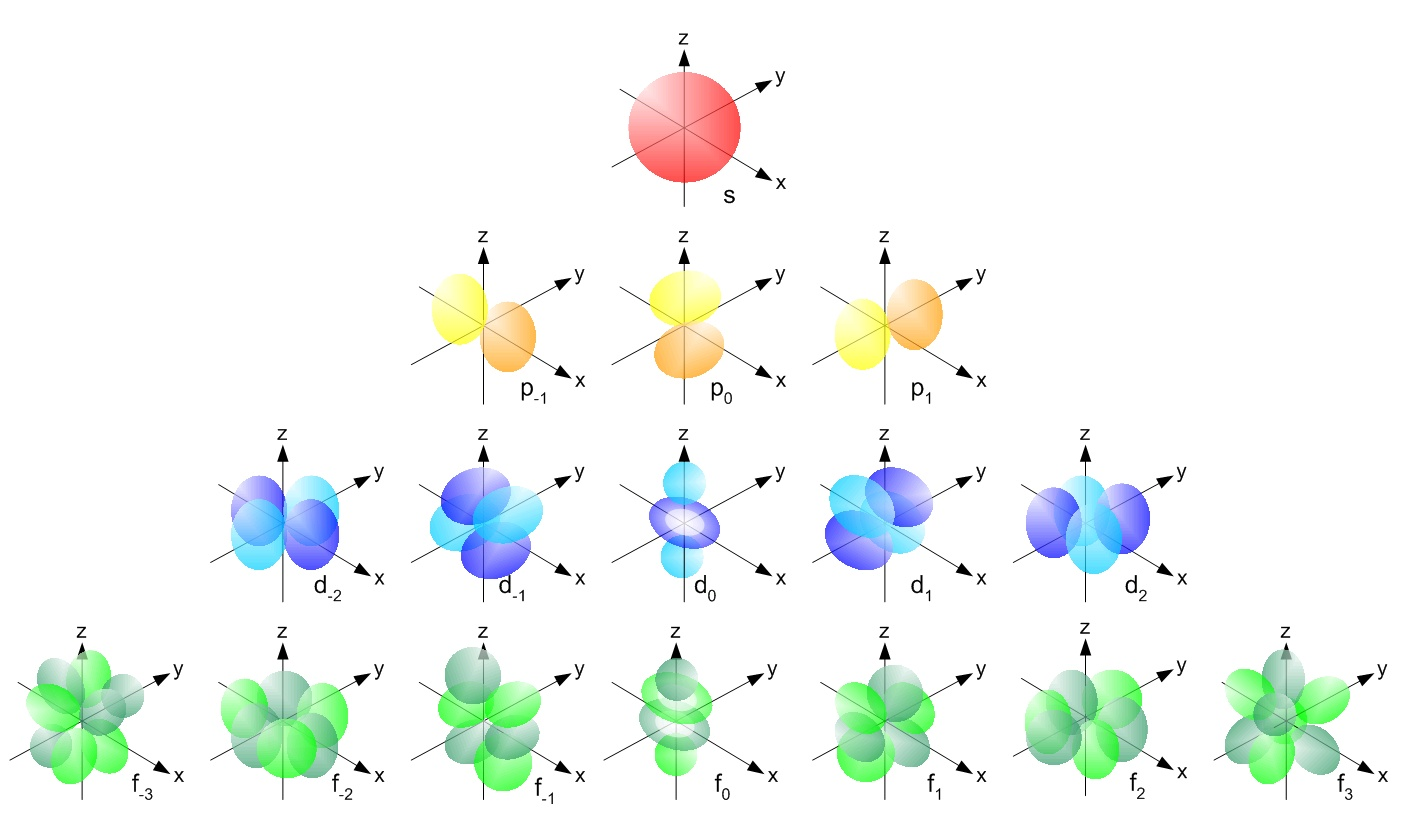
\includegraphics[width=0.8\linewidth]{single_elect_orb}
  \begin{itemize}
  \item Specific orbitals occupy certain \textbf{principal energy level} e.g.
    $n = 1, 2, 3, \cdots$
  \item Basis in which atoms form bond e.g. atomic orbitals combine
  \end{itemize}
\end{frame}

\begin{frame}{Orbital Diagram - Hydrogen}
  \centering
  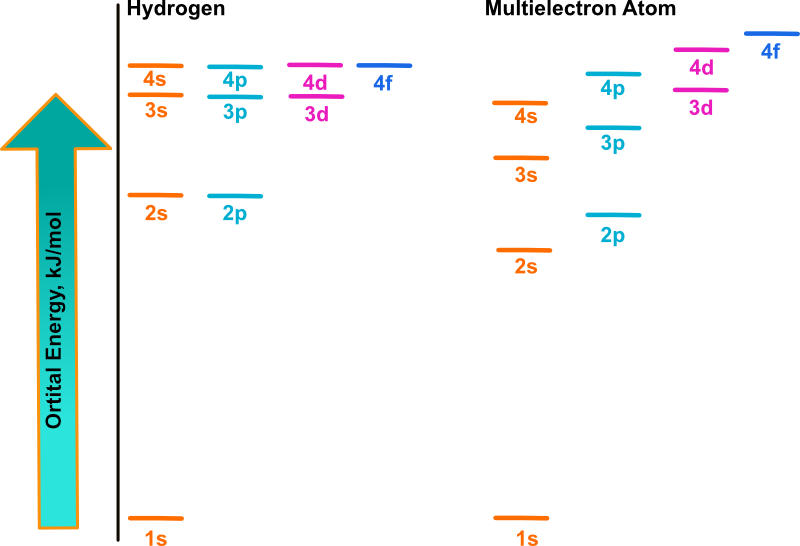
\includegraphics[scale=1.5,trim={0 0 1.2in 0},clip]{orbital_energy}
\end{frame}

\begin{frame}{Orbital Diagram - Multielectron Element}
  \textbf{Q:} What do notice about the relative atomic orbital energies?
  
  \centering
  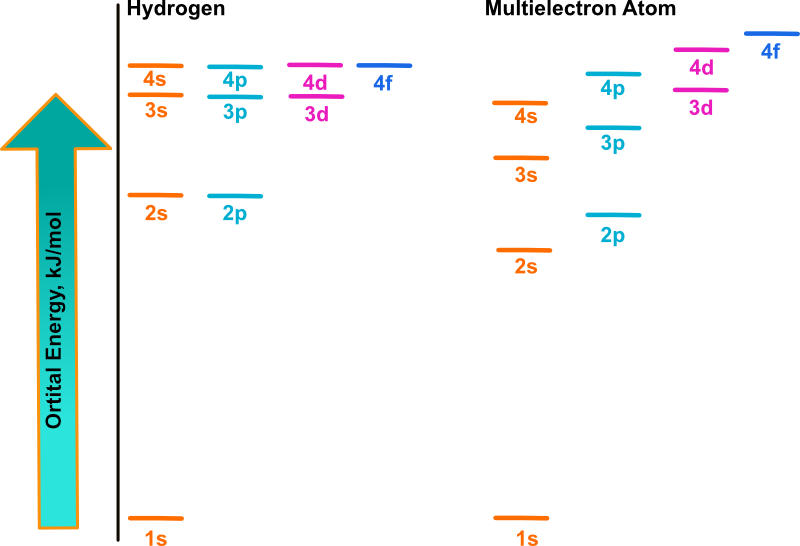
\includegraphics[scale=1.3]{orbital_energy}
\end{frame}

\begin{frame}{Principles for Filling Atomic Orbitals}
  \textbf{Aufbau principle} - electrons fill an orbital starting with
  the lowest energy level

  \textbf{Pauli exclusion principle} - No two electrons with the same
  spin can occupy the same orbital

  \textbf{Hund's Rule} - Maximize the number of unpaired electrons
\end{frame}

\begin{frame}{Relating to Periodic Table}
  \centering
  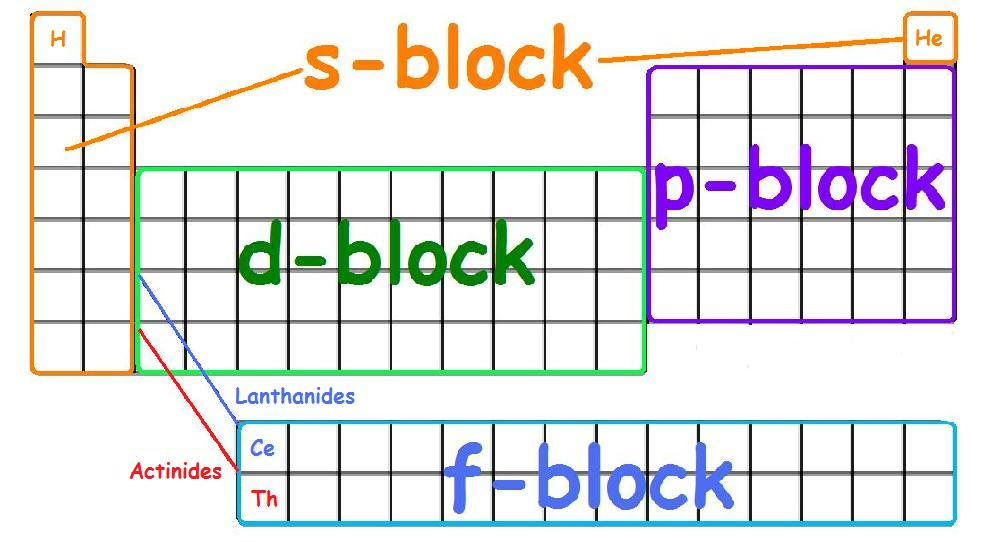
\includegraphics[width=\linewidth]{spdf_orbitals}
\end{frame}

\begin{frame}{Examples: Write Electron Configurations}
  \textbf{N}
  \vspace{0.25in}
  
  \textbf{F}
  \vspace{0.25in}
  
  \textbf{Ne}
  \vspace{0.25in}

  \textbf{Na}
\end{frame}

\begin{frame}{Purpose of Electron Configurations}
  \begin{itemize}
  \item Innermost shell is the core electrons
  \item Outermost shell is referred to as the valence
    electrons (\textbf{Q:} What is special about valence electrons?)
 \onslide<2->{\item Predicts stability of the atom e.g. half-filled or
    fully filled orbitals are stable
  }
  \onslide<3->{\item Make predictions how elements react forming new chemical
    compounds
  }
  \end{itemize}
\end{frame}

\begin{frame}{Examples: Write Electron Configurations}
  Based on the electron configurations, which atom is the most stable?
  
  \textbf{N}
  \vspace{0.25in}
  
  \textbf{F}
  \vspace{0.25in}
  
  \textbf{Ne}
  \vspace{0.25in}

  \textbf{Na}
\end{frame}

\begin{frame}{Core and Valence Electrons}
  \textbf{Core Electrons} - Energy level $n$ below the valence
  electrons and these are completely filled orbitals

  \textbf{Valence Electrons} - Outermost electrons above the energy
  level $n$ of the core electrons

  \textbf{Example:} Si - $1s^22s^22p^63s^23p^2$
\end{frame}

\begin{frame}{Practice: Writing Electron Configurations}
  Determine the atomic orbitals that contain the core and valence electrons.
  
  \textbf{Br}
  \vspace{0.25in}
  
  \textbf{Mg}
  \vspace{0.25in}
  
  \textbf{P}
  \vspace{0.25in}

  \textbf{S}
\end{frame}

\begin{frame}{Special Note about d-orbitals}
  Energy levels of 4s and 3d are close along with subsequent $n$ levels
  e.g. 5s and 4d, 6s and 5d
  
  \centering
  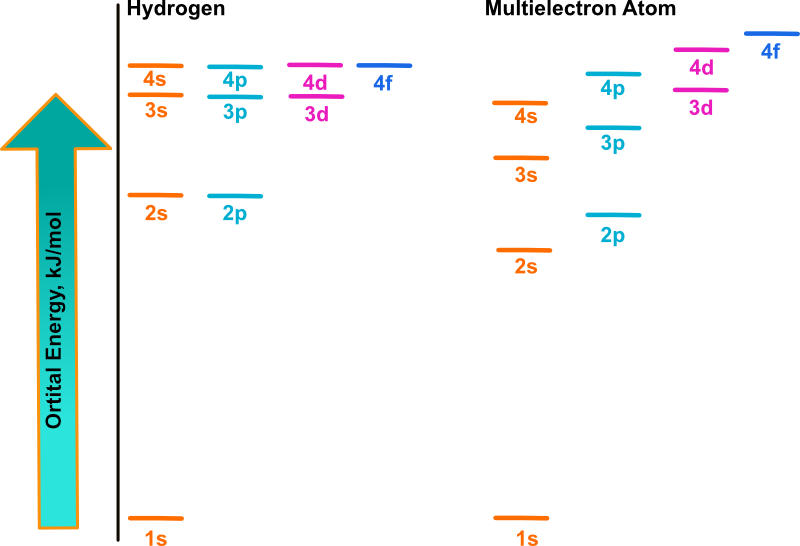
\includegraphics[scale=1.3]{orbital_energy}
\end{frame}

\begin{frame}{Relating to Periodic Table}
  \centering
  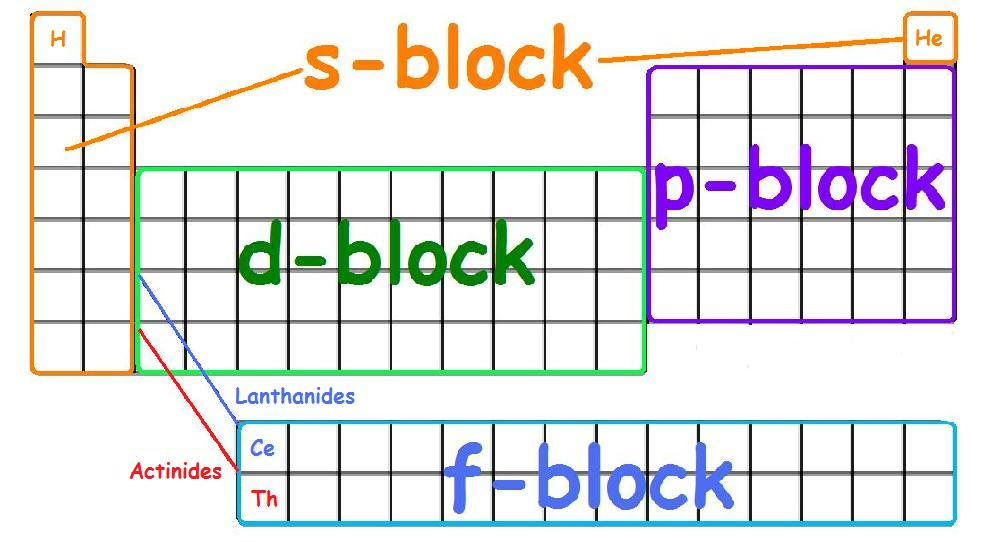
\includegraphics[width=\linewidth]{spdf_orbitals}
\end{frame}

\begin{frame}{Practice: Electron Configuration of Transition Metals}
  \textbf{Cr}
  \vspace{0.25in}
  
  \textbf{Mo}
  \vspace{0.25in}
  
  \textbf{W}
  \vspace{0.25in}

  \textbf{Cu}
  \vspace{0.25in}

  \textbf{Ag}
  \vspace{0.25in}

  \textbf{Au}
  \vspace{0.25in}
\end{frame}

\begin{frame}{Electron Configuration of Ions}
  \textbf{Q:} What is a cation? What is an anion?

  \onslide<2->{\begin{center}
    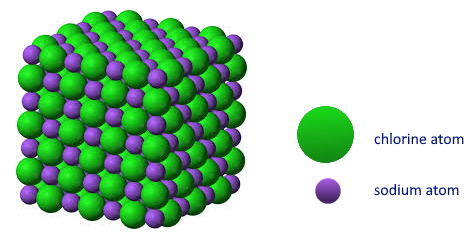
\includegraphics[width=0.7\linewidth]{nacl}
    \end{center}
    
    \textbf{Cation:} Sodium ion (Na$^+$) \textbf{Anion:} Chloride
    ion (Cl$^-$)
  }

  \onslide<3->{\textbf{Q:} For electron configuration, how do we add/remove
    electrons from atomic orbitals for anion/cation?
  }
\end{frame}

\begin{frame}{Principles for Filling Atomic Orbitals}
  \textbf{Aufbau principle} - electrons fill an orbital starting with
  the lowest energy level
  
  \textbf{Pauli exclusion principle} - No two electrons with the same
  spin can occupy the same orbital

  \textbf{Hund's Rule} - Maximize the number of unpaired electrons
\end{frame}

\begin{frame}{Practice: Writing Electron Configurations}
  \textbf{F$^-$}
  \vspace{0.25in}

  \textbf{Al$^{3+}$}
  \vspace{0.25in}

  \textbf{Na$^+$}
  \vspace{0.25in}

  \textbf{Fe$^{3+}$}
  \vspace{0.25in}

  \textbf{S$^{2-}$}
\end{frame}

\section{Periodic Properties of Atoms}

\begin{frame}{Meaning of Ionization}
  \textbf{Ionization energy} - Energy required to eject an electron
  
  \begin{center}
    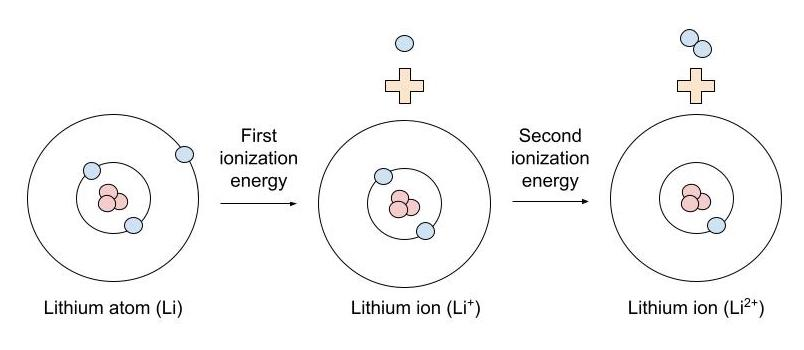
\includegraphics[width=0.8\linewidth]{ionization_Li}
  \end{center}

  First ionization takes 520 kJ/mol and second ionization takes
  7298 kJ/mol

  \onslide<2->{\textbf{Q:} Why is the second ionization energy significantly higher?}
\end{frame}

\begin{frame}{First Ionization Energy Trends}
  \centering
  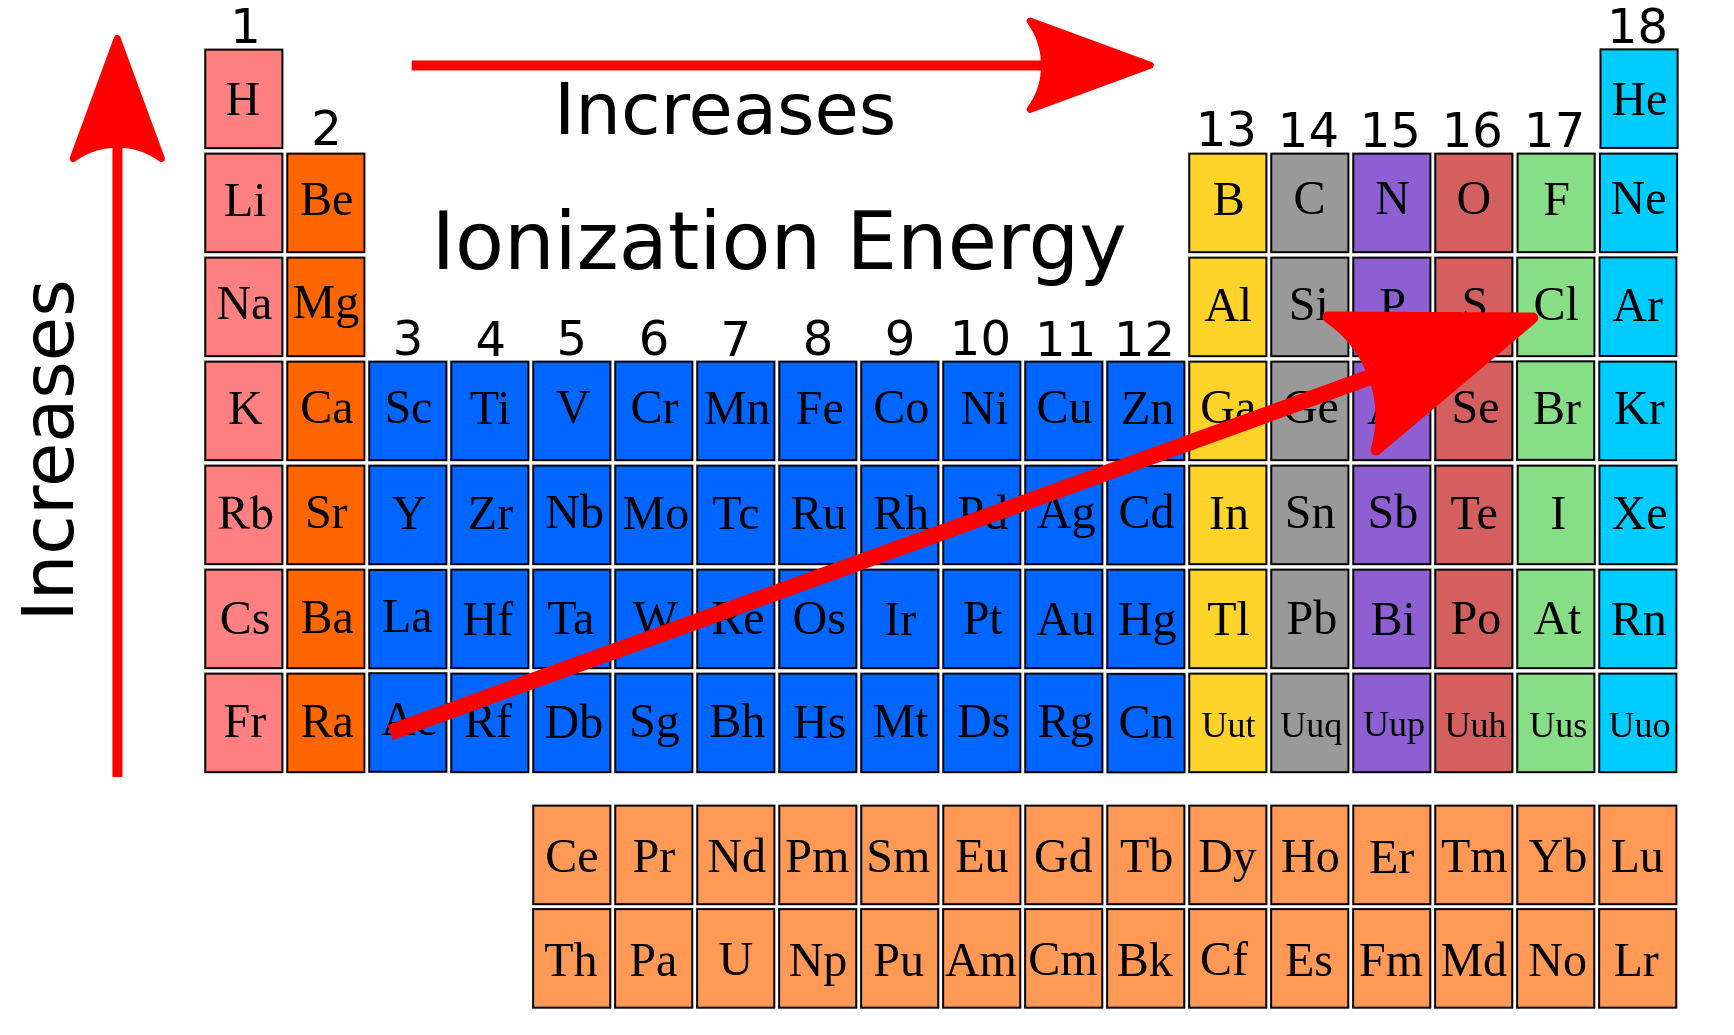
\includegraphics[width=\linewidth]{ion_trends}
\end{frame}

\begin{frame}{First Ionization Energy Trends}
  \centering
  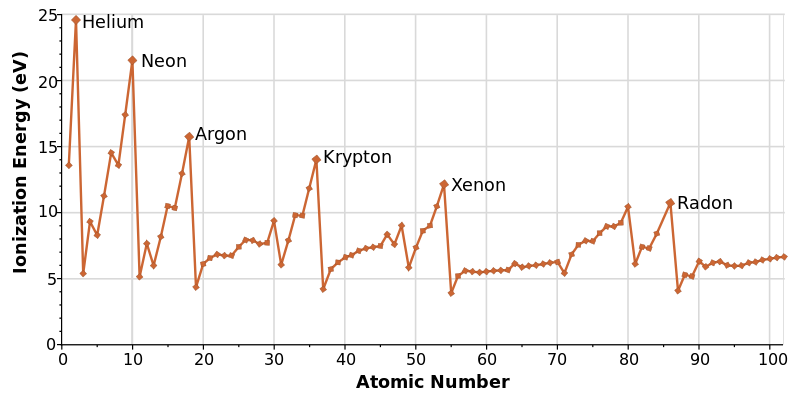
\includegraphics[width=\linewidth]{first-ionization-energy}
\end{frame}

\begin{frame}{Atomic Sizes of Neutral Atoms}
  \centering
  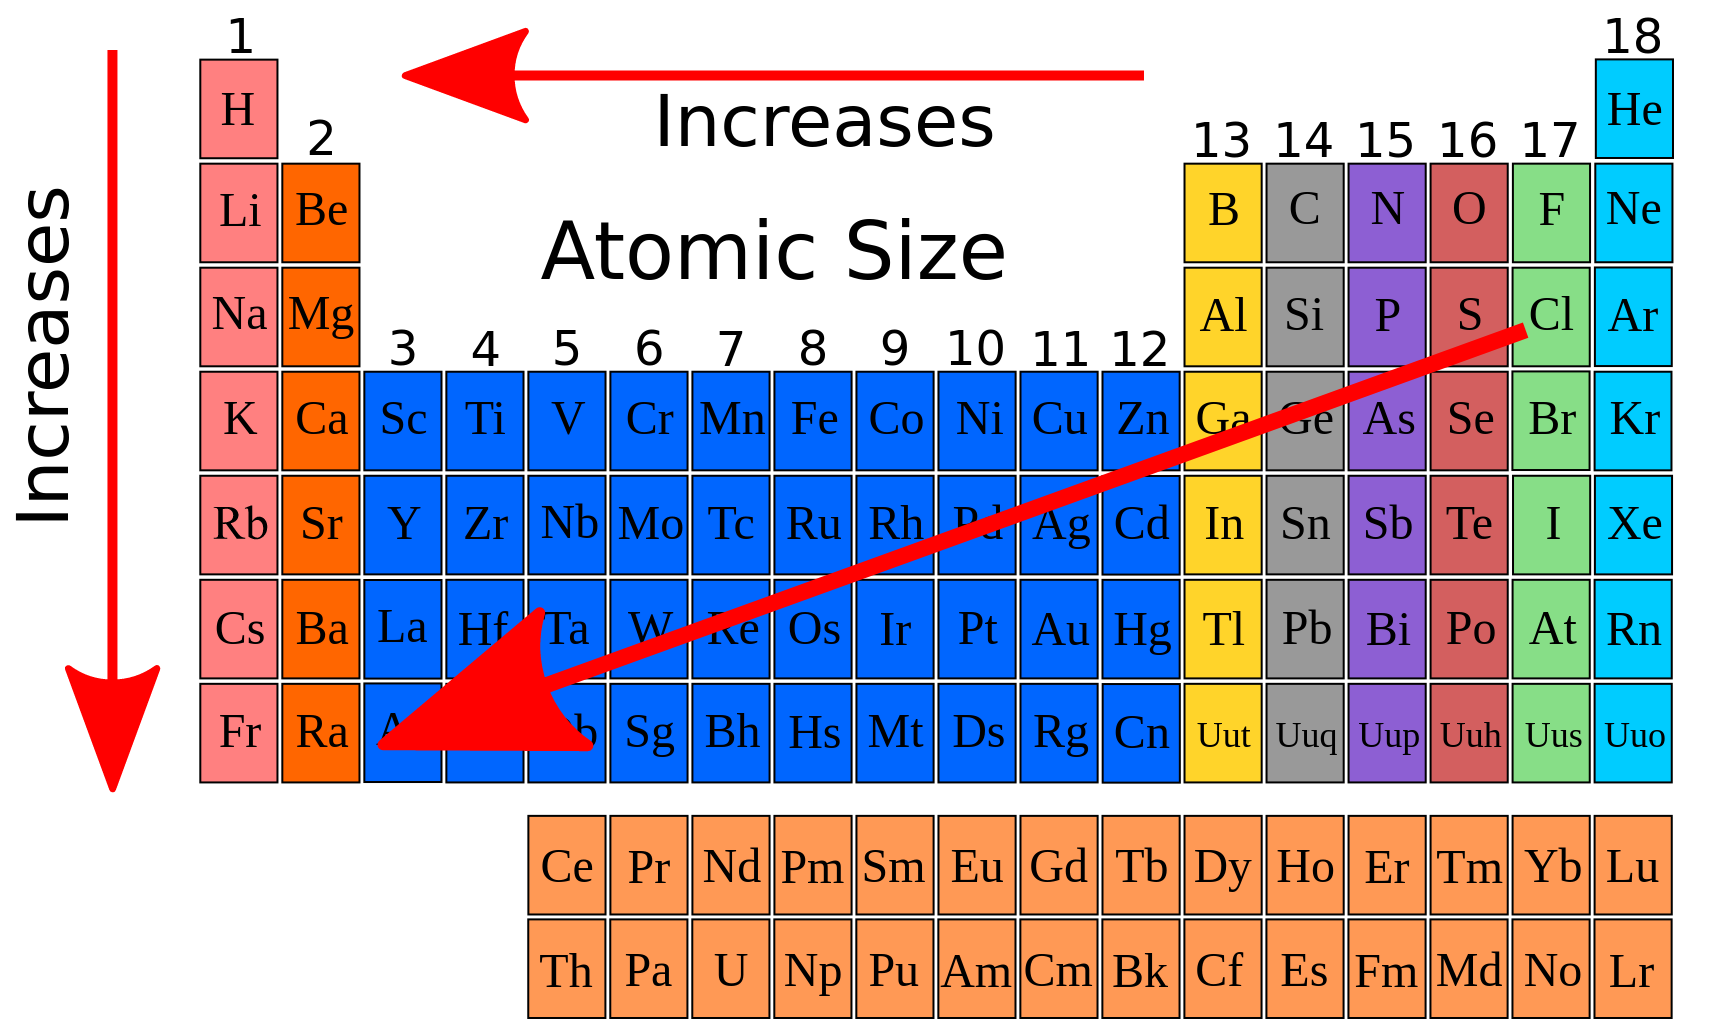
\includegraphics[width=\linewidth]{atomic_trend}
\end{frame}

\begin{frame}{Atomic Sizes of Neutral Atoms}
  \centering
  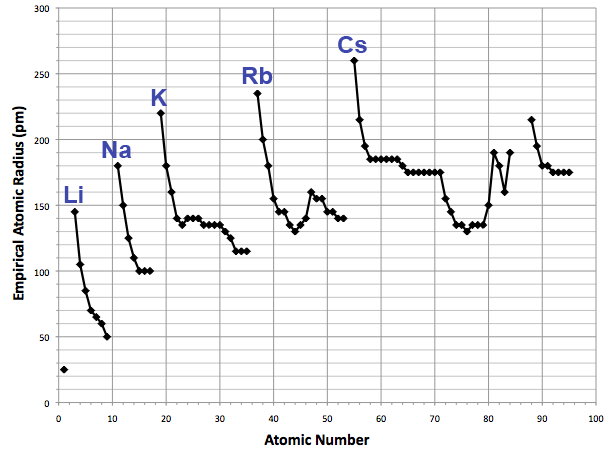
\includegraphics[width=\linewidth]{graph_atomic_rad}
\end{frame}

\begin{frame}{Atomic Sizes of Ions}
  \centering
  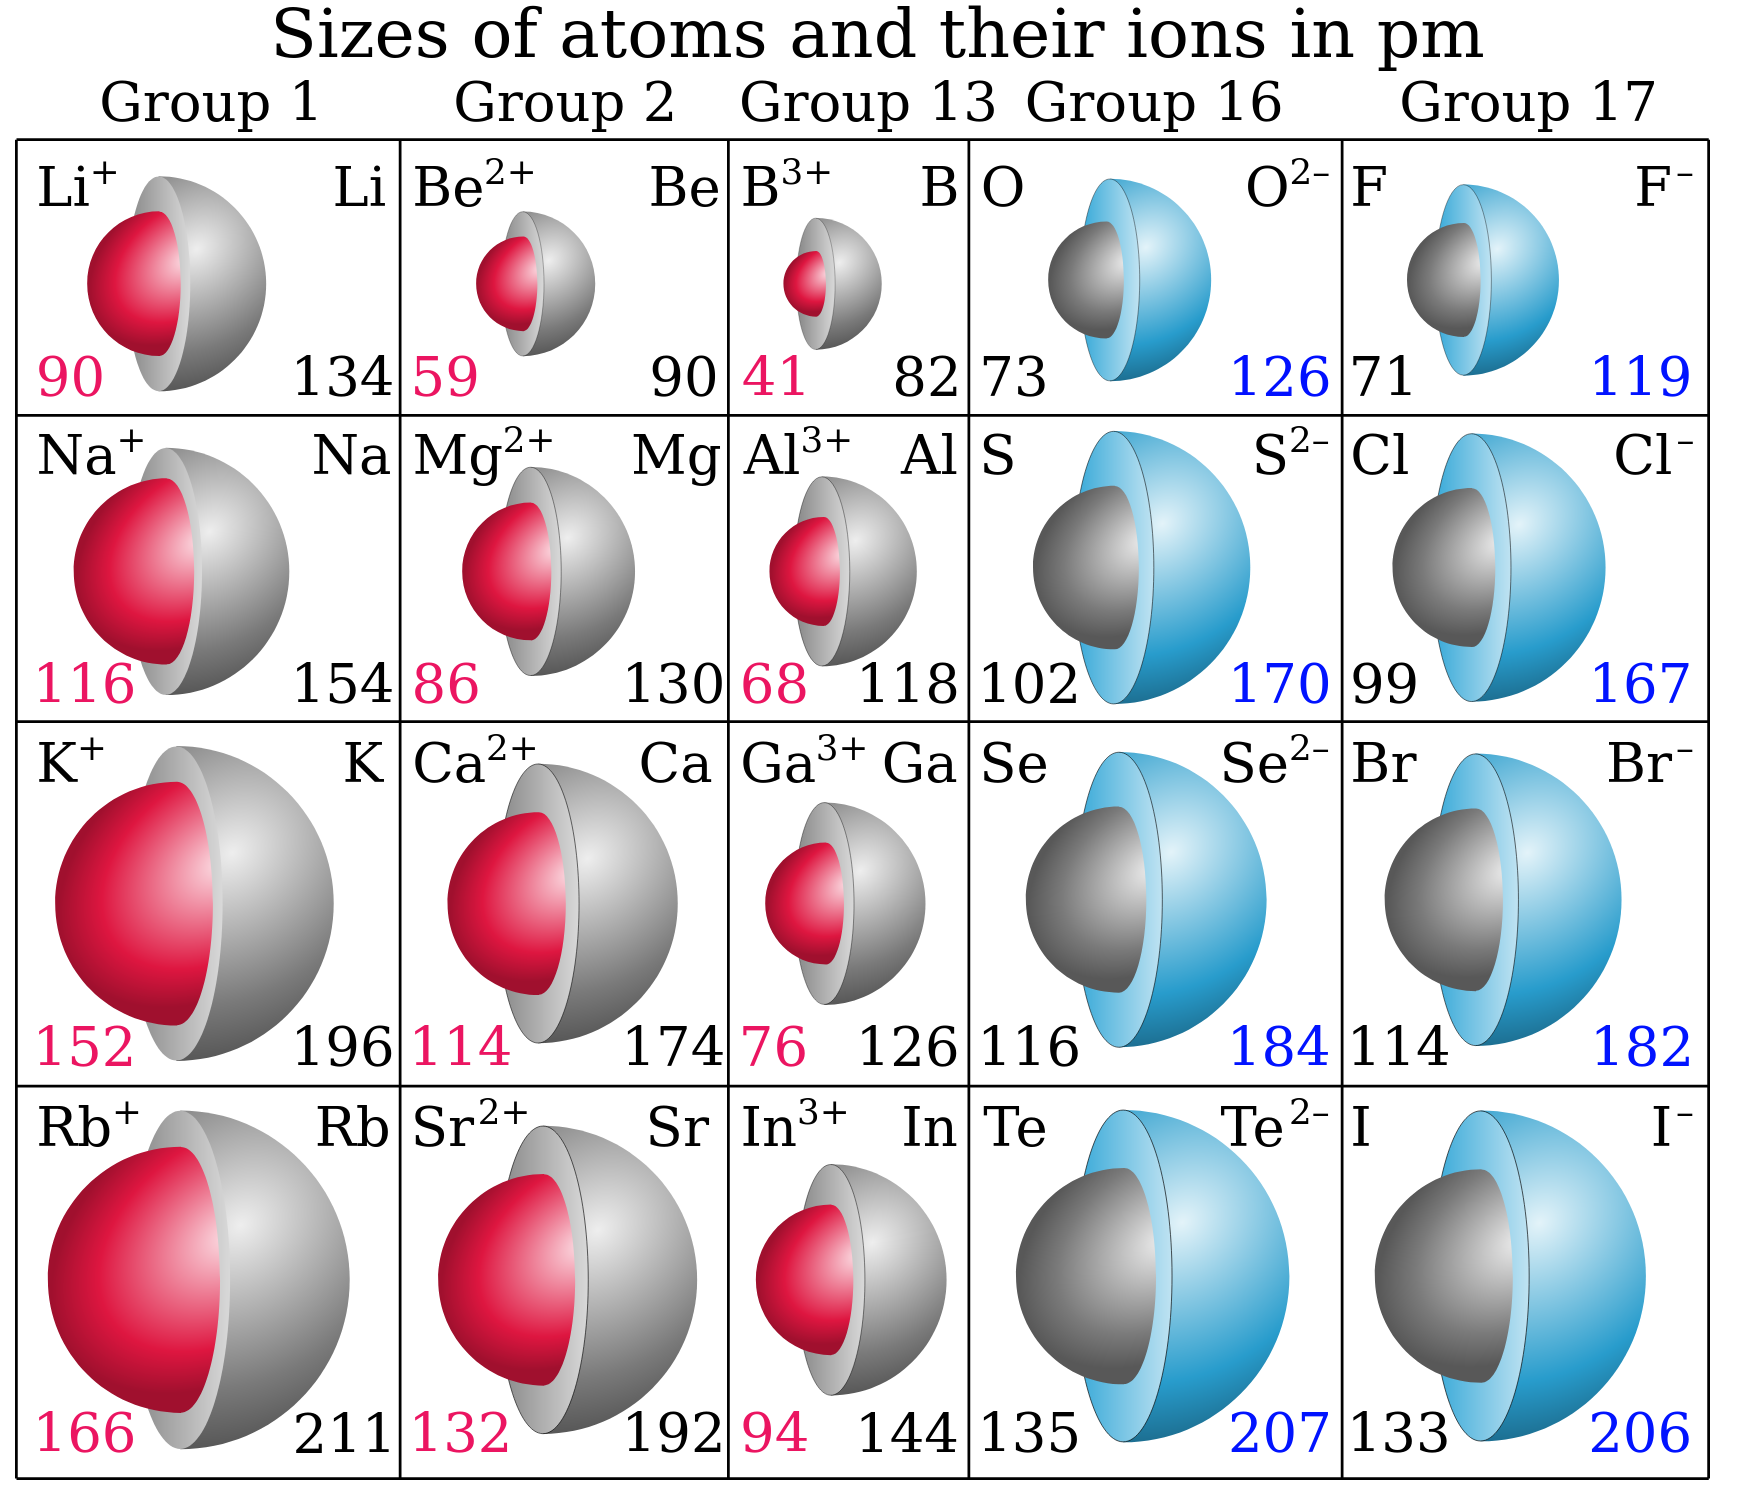
\includegraphics[width=0.8\linewidth]{ion_radii}
\end{frame}

\end{document}
